%%%%%%%%%%%%%%%%%%%%%%%%%%%%%%%%%%%%%%%%%%%%%%%%%%%%%%%%%%%%%%%%%%%%%%%%%%%%%%%
% Chapter 3: Procedimiento experimental 
%%%%%%%%%%%%%%%%%%%%%%%%%%%%%%%%%%%%%%%%%%%%%%%%%%%%%%%%%%%%%%%%%%%%%%%%%%%%%%%

Este cap�tulo ha de contar con seccciones para la descripci�n de los experimentos 
y del material.
%
Tambi�n debe haber una secci�n para los resultados obtenidos y una �ltima de 
an�lisis de los resultados.

%++++++++++++++++++++++++++++++++++++++++++++++++++++++++++++++++++++++++++++++
\section{Descripci�n de los experimentos}
\label{3:sec:1}
A continuaci�n expondremos los pasos que se han seguido en la elaboraci�n del experimento desarrollado para este trabajo de investigaci�n. 
Nos apoyaremos en gr�ficos y tablas que les ayudaran a reforzar y aclarar la informaci�n desarrollada.
\subsection{Descripci�n de los experimentos}
Para llevar a cabo el m�todo de {\em Taylor}, objetivo principal del informe, se ha empleado la ecuaci�n del m�todo de {\em Taylor}. Recodar que  la funci�n derivada ha sido $f(x)=arcsin(x)$  y que al aplicar la serie de Taylor hemos tenido que calcular hasta la derivada n-�sima y, adem�s, elos factoriales de 1 hasta n.

En relaci�n a la eficiencia del proyecto, se ha analizado el resultado obtenido de la aproximaci�n de Taylor midiendo el error de este con el resultado original de la funci�n. 

%++++++++++++++++++++++++++++++++++++++++++++++++++++++++++++++++++++++++++++++
\section{Descripci�n del material}
\label{3:sec:2}
El material utilizado ha sido el siguiente:
\begin {itemize}
\item \underline{Tipo de CPU}: 
 
 
 Intel(R) Core(TM) i3-2328M CPU @ 2.20GHz 

\item \underline{Tama�o de la memoria del procesador}: 


 3072 KB

\item \underline{Vendedor GenuineIntel}:


Linux

\item \underline{Sistema operativo}:


 66-Ubuntu SMP

\item \underline{Plataforma}:


 Linux-3.2.0-59-generic-pae-i686-with-Ubuntu-12.04-precise

\item \underline{Version}:

2.7.3
\end{itemize}


%++++++++++++++++++++++++++++++++++++++++++++++++++++++++++++++++++++++++++++++

\section{Resultados obtenidos}
\label{3:sec:3}
Como resultados de haber  calculado en el algoritmo para cualquiero polinomio obetemos el valor del polinomio con el m�todo de Taylor, el error y el tiempo\footnote{En segundos}  que tarda el algoritmo en calcularlos.


Como ejemplos de los tiempos y errores en diferentes puntos de un polinomio de grado 3, obtenemos representado en la tabla:
\newpage
%------------- c----------------------------------------------------------------
%--------------------------------------------------------------------------
\begin{table}[!ht]
\begin{center}
\begin{tabular}{|c|c|} \hline 
\textbf{Tiempo  } & \textbf{Velocidad} \\ 
\textbf{($\pm$ 0.001 s)} & \textbf{($\pm$ 0.1 m/s)} \\ \hline \hline
1.234 &
67.8
\\
\hline

2.345 &
78.9
\\
\hline

3.456 &
89.1
\\
\hline

4.567 &
91.2
\\
\hline

\end{tabular}
\end{center}
\caption{Resultados experimentales de tiempo (s) y velocidad (m/s)}
\label{tab:1}
\end{table}


%------------------------------------------------------------------------------
Por cada dato que calculamos obtemos la funci�n representada en una gr�fica en dicho punto, como por ejemplo esta gr�fica:
%------------------------------------------------------------------------------
\begin{figure}[!th]
\begin{center}
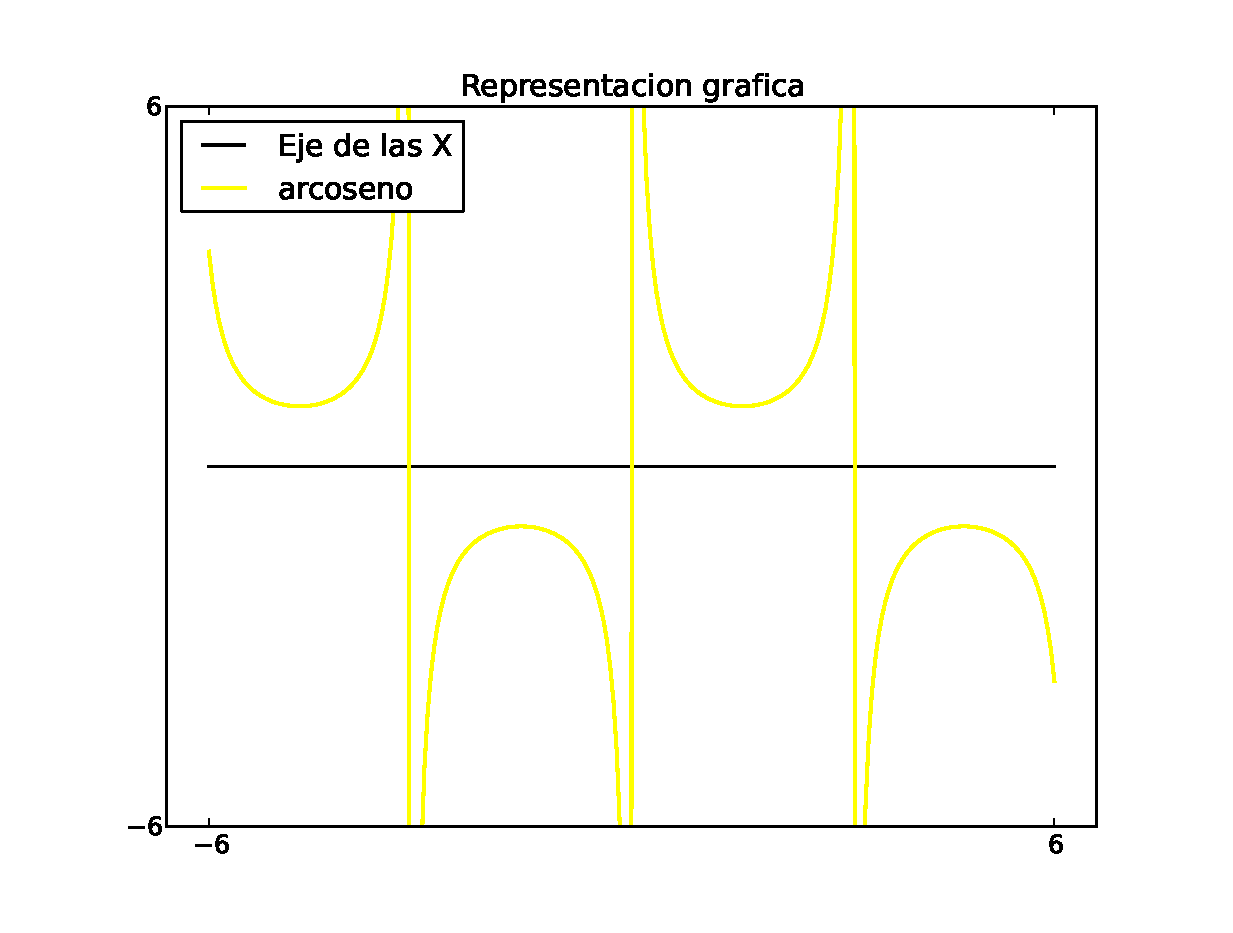
\includegraphics[width=0.75\textwidth]{images/grafica.eps}
\caption{Gr�fica de la funci�n arcsin(x)}
\label{fig:1}
\end{center}
\end{figure}
%------------------------------------------------------------------------------
%++++++++++++++++++++++++++++++++++++++++++++++++++++++++++++++++++++++++++++++
\section{An�lisis de los resultados}
\label{3:sec:4}
